\documentclass[11pt]{report}
\usepackage[french]{babel}
\usepackage[utf8]{inputenc}
\usepackage[T1]{fontenc}
\usepackage[top = 2cm, bottom = 2cm, left = 1cm, right = 1cm]{geometry}
\usepackage{fancyvrb}
\usepackage{mathalfa}
\usepackage{amsfonts}
\usepackage[table]{xcolor}
\usepackage{amsmath}
\usepackage{graphicx}
\usepackage{listings}
\usepackage{color}
\usepackage{comment}
\usepackage{times}
\usepackage[hidelinks]{hyperref}
\usepackage{parskip}

\begin{document}

\setcounter{secnumdepth}{3}
\setcounter{tocdepth}{3}
\title{Cahier des charges projet IA04 : Flotte de drones en 2D}
\date{}
\renewcommand{\thesection}{\arabic{section}}
\maketitle
\renewcommand{\contentsname}{\centering Sommaire}
\tableofcontents

\newpage
\section{Présentation globale de l'idée}
\subsection{Définition d'un drone}

\textit{Un drone (de l'anglais drone) désigne un aéronef sans pilote à bord. Le drone peut avoir un usage civil ou militaire. [...] Sa taille et masse (de quelques grammes à plusieurs tonnes) dépendent des capacités recherchées. Le pilotage automatique ou à partir du sol permet des vols longs de plusieurs dizaines d'heures (à comparer aux deux heures typiques d'autonomie d'un chasseur).} - Wikipédia :  \textcolor{blue}{\url{https://fr.wikipedia.org/wiki/Drone}}

\subsection{Modélisation}

On suppose qu'un agent représente un drone et on se place dans un plan 2D ($xOy$). Chaque drone est assimilé à un point qui représente sa position $(x, y)$ dans le plan. L'objectif est de faire en sorte que les agents coexistent dans un périmètre donné. Les coordonnées sont positives, on se place dans $\mathbb{R}^{2}_{+}$. L'espace de déplacement (l'environnement) n'est pas torique et est limité par des bornes en $x$ et $y$. L'espace n'est pas forcément carré.

\subsection{Comportement des drones}

La coexistence des drones est basée sur plusieurs règles de fonctionnement : 

\begin{enumerate}
\item Les drones ont tendance à s'organiser en flotte, le nombre de drones maximal dans une flotte est une constante à définir au début du programme.

\item Les drones sont démarrés seuls au départ et ne font pas partie d'une flotte.

\item Chaque drone a un unique identifiant (qui dans JADE je suppose correspondra en fait à son AID).

\item Chaque flotte a un un maître qui guide sa flotte.

\item Les flottes sont en anneau, le diamètre peut varier en fonction des objets ou autres drones sur leur passage, de manière donc à éviter les collisions.

\item La communication des drones se fait par ondes radio à courte portée, ce qui concrètement veut dire qu'un drone ne peut émettre qu'à un certain rayon autour de lui, et de même ne recevoir qu'à une distance inférieure ou égale à ce rayon.

\item Lorsqu'un drone (ou une flotte) rencontre un autre drone (ou une autre flotte), une procédure est activée de manière à ce que les deux ensembles fusionnent (ou non, en fonction du nombre de drones déjà présents dans la flotte).

\item Lorsqu'un drone est détruit (par exemple il s'écrase contre un bâtiment, représenté par un polygone sur le plan), il est retiré du graphique (le point qui le représentait est effacé).

\item Inversement lorsqu'un drone est créé, le point le représentant apparait sur le graphique.

\item La communication utilisée dans une flotte est une communication de proche en proche (topologie en anneau) : \url{https://fr.wikipedia.org/wiki/Topologie_de_reseau#Le_r.C3.A9seau_en_anneau}
\end{enumerate}

\newpage
\subsection{Objectif}

L'idée est donc de modéliser ce système et d'y incorporer une \textbf{interface graphique} (animation) afin de visualiser en temps réel les déplacements et les différents interactions des drones.

Voici une image de ce à quoi cela pourrait ressembler (ce serait donc une capture à un instant donné de la figure graphique) : 

\begin{figure}[h]
\centering
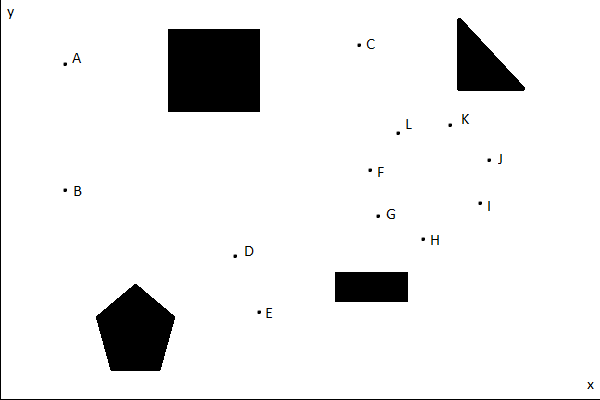
\includegraphics{img/drones-graphique.png}
\caption{Les points $A$, $B$, ... sont des drones et les polygones noirs sont des objets (facultatif)}
\end{figure}

\clearpage
\section{Implémentation}
\subsection{Architecture JADE}

L'architecture se divise en trois parties : les drones qui évoluent dans l'environnement 2D, les objets qui se trouvent sur le terrain, et l'interface graphique qui va représenter tout cela sur l'écran. Ces trois parties sont plus ou moins indépendantes.

\subsection{La classe \protect\Verb+Drone+}
\subsubsection{Description}

La classe \verb|Drone| est la principale classe à implémenter. En termes de cardinalité, le nombre d'instances de cette classe peut varier de $1$ à $n$.

\subsubsection{Attributs}

La liste d'attributs de la classe \verb|Drone| :

\begin{enumerate}
\item La position actuelle du drone dans le plan $p = (x, y)$ qui est représentée par une instance d'une classe à définir, qui définira un certain nombre de méthodes (par exemple renvoyer la distance entre deux points du plan).

\item Un identifiant unique qui peut éventuellement être l'AID du drone.

\item Un état à définir par la suite, notamment lors des fusion de flotte, il faudra imposer aux drones de ne plus se déplacer et d'ignorer les messages reçus de l'environnement, donc il leur faudra un état particulier qui les mettra en stand-by.

\item La prochaine position du drone (calculée en fonction de la position actuelle, de la position objectif, et de l'environnement immédiat).

\item La position objectif du drone.

\item La flotte à laquelle il appartient, s'il appartient à une flotte.

\item Son rang dans la flotte et le voisin auquel il doit envoyer un message (anneau unidirectionnel), s'il appartient à une flotte.
\end{enumerate}

\subsubsection{Behaviours} 

Le drone doit pouvoir réagir à son environnement de plusieurs manières, dépendamment des stimuli qui lui parviennent. Voici la liste des behaviours de la classe \verb|Drone| :

\begin{enumerate}
\item Un behaviour qui renvoie la position de l'agent à l'agent \verb|Display| quand il le lui demande.

\item Un behaviour qui envoie spontanément un message à l'agent \verb|Display| lors de la mort de l'agent (l'agent \verb|Display| devra dans ce cas supprimer le drone de la liste des drones et mettre à jour l'affichage).

\item Un behaviour qui réagit aux messages provenant de d'autres éléments de la classe \verb|Drone|.

\item Un behaviour qui envoie périodiquement des messages dans l'environnement immédiat de l'agent (il se contente d'émettre aux autres agents, la réception du message se fera par une fonction de filtration sur l'attribut position).

\item Un behaviour qui réagit aux messages provenant des objets (dans cette modélisation, les objets sont des ensembles de points fixes dont les points périphériques envoient périodiquement des messages aux drones).
\end{enumerate}

\newpage
\subsection{La classe \protect\Verb+Display+}
\subsubsection{Description}

La classe \verb|Display| est une classe indépendante de la classe \verb|Drone|. Son rôle est de rappatrier les positions des drones et de les afficher sur une interface graphique. L'implémentation de classe passe donc par l'utilisation d'une librairie graphique Java. En termes de cardinalité, le nombre d'instances de cette classe est exactement de $1$. C'est la première classe créée lors du lancement du programme, et elle crée les autres objets dès son démarrage. Elle initialise les position des drones (qui peuvent éventuellement être passées en paramètres) et des objets.

\subsubsection{Attributs}

La liste d'attributs de la classe \verb|Display| :

\begin{enumerate}
\item Un tableau dynamique (du fait de la suppression possible de drones au cours de l'évolution de la simulation) recensant les drones existants.

\item Le nombre de drones existants.

\item Un tableau dynamique recensant les objets sur le terrain.

\item Le nombre d'objets existants.

\item La dernière représentation graphique calculée (matrice dépendant de la librairie graphique utilisée, paramètre à déterminer).
\end{enumerate}

\subsubsection{Behaviours}

Voici la liste des behaviours de la classe \verb|Display| :

\begin{enumerate}
\item Un behaviour qui envoie périodiquement à tous les agents \verb|Drone| une demande de leur position. Il met à jour le tableau de positions.

\item Un behaviour qui reçoit un signal de mort de la part d'une drone, dans ce cas il devra le supprimer de sa liste de drones.

\item Un behaviour qui répond un signal d'arrêt en provenance de la console, il supprimera tous les drones et objets et terminera l'exécution.

\item Un behaviour qui rafraîchit constamment l'interface graphique sur la base des positions actuelles des drones.
\end{enumerate}

\newpage
\subsection{La classe \protect\Verb+Object+}
\subsubsection{Description}

La classe \verb|Object| est facultative. Il faut prioriser le développement des deux classes précédentes. Si les deux classes précédentes sont terminées en avance et que la simulation fonctionne, on peut passer à cette classe. Elle représente les objets qui se trouvent sur le terrain. Les objets sont des polygones. Un objets est un ensemble de points dont les points frontaliers sont ceux qui émettent des messages.

\subsubsection{Attributs}

La liste d'attributs de la classe \verb|Object| :

\begin{enumerate}
\item Un tableau de points représentant la totalité des points qui le composent.

\item Un identifiant unique.
\end{enumerate}

\subsubsection{Behaviours}

La liste des behaviours de la classe \verb|Object| :

\begin{enumerate}
\item Un behaviour qui émet constamment des messages (destinés aux agents) dans les environs de l'objet. Seuls les points frontaliers doivent émettre des messages. Il faudra donc une méthode de classe qui définit la frontière de l'objet.

\item Un behaviour qui renvoie l'ensemble des points le constituant à l'agent \verb|Display| lorsqu'il le lui demande.
\end{enumerate}

\newpage
\section{Communication des drones}

Dans cette partie, on va définir les différents cas de figure qui peuvent se présenter dans la vie d'un drone et l'implémentation et les algorithmes qui en découlent. On définira également d'un point de vue technique la nature des messages échangés et l'état des drones au cours de ces situations.

\subsection{Déplacement sans flotte}
.
\subsection{Crash contre un objet}
.
\subsection{Croisement d'un drone seul}
.
\subsection{Croisement d'un drone ayant une flotte}
.
\subsection{Intégration d'un drone dans une flotte}
.
\subsection{Fusion de deux flottes}
.
\subsection{Destruction d'un élément de la flotte}
.
\subsection{Déplacement en flotte}
.
\end{document}